\chapter{\IfLanguageName{dutch}{Stand van zaken}{State of the art}}%
\label{ch:stand-van-zaken}

% Tip: Begin elk hoofdstuk met een paragraaf inleiding die beschrijft hoe
% dit hoofdstuk past binnen het geheel van de bachelorproef. Geef in het
% bijzonder aan wat de link is met het vorige en volgende hoofdstuk.

% Pas na deze inleidende paragraaf komt de eerste sectiehoofding. 
% TODO - Inleiding - OK

Tegenwoordig is samenwerken in teamverband een belangrijk aspect op de werkvloer. Om projecten succesvol af te ronden, is goede communicatie binnen het team en een efficiënte manier van werken essentieel. Om dit proces te vergemakkelijken, maken veel organisaties gebruik van online tools zoals Podio of gelijkaardige platformen. Deze platformen worden ook wel low-code/no-code development platformen genoemd, maar wat houd dit precies in? Wat is doet Podio nu precies en wat kan er allemaal mee bereikt worden? \\
 
In de stand van zaken wordt eerst en vooral toegelicht wat een no-code/low-code development platform precies is en waar de term vandaan komt. Vervolgens komen ook de interne verschillen en de uitdagingen voor dit type platformen aan bod. Daarna wordt wat dieper ingegaan op de platformen die in deze studie aan bod zullen komen, namelijk Podio, Airtable en Google Appsheet. Er wordt overlopen hoe ze ontstaan zijn en welke mogelijkheden ze allemaal te bieden hebben. \\

\section{Low-code/no-code Development Platforms} 
\label{sec:low_code}

\subsection{Geschiedenis van Low-code development}
\label{subsec:geschiedenis_low_code}
% https://link.springer.com/article/10.1007/s10270-021-00970-2
% Supporting-the-understanding-and-comparison-of-low-code-development-platforms.pdf

Eerst en vooral is het belangrijk om toe te lichten wat er verstaan wordt onder de term 'low-code development platform'. Zoals weergegeven in figuur \ref{fig:lcdp_history} dateert de eerste vermelding van de term \textit{low-code} in 2014. Toen werden ze gedefinieerd als `platformen die een snelle oplevering van business applicaties toestaan, met een minimum aan handgeschreven code en investering in setup, training en deployment` \autocite{Ruscio2022}. In 2017 werd deze definitie echter bijgewerkt tot een meer gedetailleerde variant, low-code development platforms (LCDP's) werden omschreven als `product en/of cloud services voor het ontwikkelen van applicaties die visuele, declaratieve technieken gebruiken in plaats van programmeren en die toegankelijk zijn tot gebruikers voor een minimum van training of kosten` \autocite{Ruscio2022}. \\

\begin{figure}[h]
    \centering
    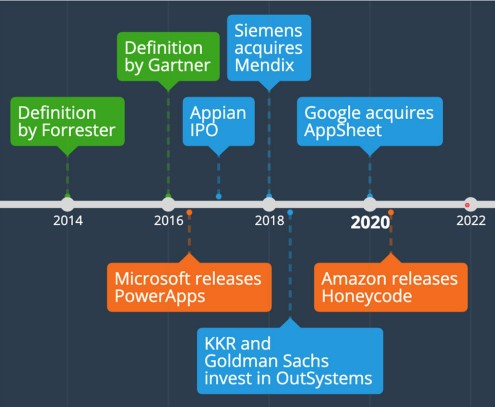
\includegraphics{LCDP_MajorEvents.jpg}
    \caption{Korte historie van low-code development platforms \autocite{Ruscio2022}.}
    \label{fig:lcdp_history}
\end{figure}

\subsection{Wat is een low-code development platform?}
\label{subsec:what_is_low_code}

Een low-code platform wordt door \textcite{Waszkowski2019} omschreven als 'Een set van tools voor programmeurs en niet-programmeurs'. In dit type development platform wordt gesteund op een grafische user interface (GUI) voor het ontwerpen en bouwen van applicaties. Het stelt de gebruiker in staat om snel en met weinig programmeerkennis, een volledige business applicatie op te bouwen. \\

In het algemeen bestaan low-code platformen uit vier lagen, zoals weergegeven in figuur \ref{fig:lcdp_structure}. De bovenste laag of Application Layer bevat de GUI waarmee de gebruiker gaan interageren om hun gewenste applicatie op te bouwen. Daarbovenop bevat deze laag de authenticatie en autorisatie mechanismen. De tweede laag of Service Integration Layer maakt verbinding met verschillende diensten aan de hand van API's en authenticatiemechanismen. Vervolgens is er de Data Integration Layer, deze houdt zich bezig met de integratie van gegevens uit verschillende bronnen. Ten slotte is er nog de Deployment Layer die de ontwikkelde applicatie zal opzetten in speciale cloud infrastructuren of on-premise omgevingen, waarbij containerisatie, orkestratie en continue integratie en deployment (CI/CD) gefaciliteerd worden. \\

\begin{figure}[ht]
    \centering
    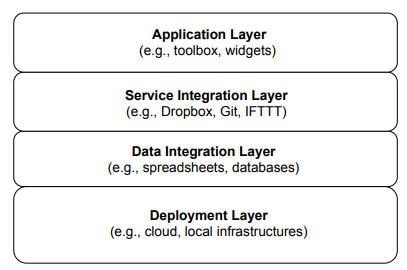
\includegraphics[width=\linewidth]{LCDP_Structure.png}
    \caption{Algemene structuur van low-code development platforms \autocite{Sahay2020}.}
    \label{fig:lcdp_structure}
\end{figure}

De ontwikkeling van een applicatie aan de hand van LCDP's verloopt in verschillende stappen, die in een studie van \textcite{Ruscio2022} uitgebreid worden besproken. In de eerste fase definiëren gebruikers de concepten en relaties in de applicatie om op die manier het domein te modelleren. Dit gebeurt meestal met behulp van modelleer constructen zoals drag-and-drop die door het platform worden meegeleverd. In de volgende fase, de specificatie van businesslogica, worden de controle- en gegevensstromen van het systeem gedefinieerd zoals grafische workflows. LCDP's voorzien ook interoperabiliteit met externe services en datasources, zodat gebruikers kunnen verbinden en integreren met systemen van derden. Zodra de gewenste applicatie is gespecificeerd en gebouwd, kan het worden gedeployed in een publieke of private omgeving. Vaak gaat deze deployement door in cloud-infrastructuren. De laatste fase is het onderhouden van de applicatie, in de meeste gevallen heeft een low-code development platform features om te reageren op onvoorziene requirements of problemen die kunnen voorkomen terwijl de applicatie online staat . \\

\subsection{Verschillen tussen low-code en no-code}
\label{subsec:verschillen_low_code}

No-code en low-code development platformen zijn op zich heel gelijkaardig aan elkaar, beide stellen namelijk een gebruiker in staat om applicaties te ontwikkelen met weinig tot geen code. Toch zijn er enkele kleine verschillen tussen beide, deze verschillen gaan vooral over wat mogelijk is en wat niet mogelijk is bij elk type \autocite{Yan2021}. Ten eerste zijn low-code platformen in het algemeen meer complex dan no-code platformen, waardoor er meer technische kennis nodig is om ze goed te gebruiken. Daarnaast bieden ze ook meer opties bij het personaliseren van een applicatie en laten ze toe om meer geavanceerde applicaties te bouwen. Verder gaan low-code platformen meestal eenvoudiger te integreren zijn met bestaande systemen, omdat ze flexibeler zijn. Kortom hebben zowel no-code als low-code development platforms hun voordelen en nadelen. Welk platform een organisatie gebruikt, hangt dus vooral af van hun specifieke behoeften en technische expertise \autocite{Yan2021}.

\subsection{Uitdagingen voor no-code/low-code development}
\label{subsec:uitdagingen_low_code}

No-code en low-code ontwikkeling zijn de laatste jaren steeds populairder geworden omdat ze non-IT-professionals in staat stellen snel eenvoudige business applicaties te bouwen zonder of met weinig codering \autocite{Yan2021}. Toch zijn er nog enkele uitdagingen verbonden aan deze methode van development. \\

\begin{itemize}
    \item \textbf{Beperkte aanpasbaarheid}: No-code/low-code platformen maken vaak gebruik van vooraf gebouwde componenten of templates. Hierdoor wordt de vrijheid voor het personaliseren van een applicatie beperkter \autocite{Yan2021}.
    \item \textbf{Beperkte functionaliteit}: Hoewel deze platformen kunnen worden gebruikt om eenvoudige applicaties te bouwen, zijn ze mogelijk niet geschikt voor complexere applicaties die geavanceerde functionaliteiten vereisen \autocite{Yan2021}.
    \item \textbf{Integratie met andere systemen}: Indien een systeem niet ontworpen is om te werken met no-code/low-code applicaties, kan het integreren een enorme uitdaging zijn \autocite{Ferreira2019}.
    \item \textbf{Beveiligingsproblemen}: No-code/low-code platformen voorzien mogelijks niet hetzelfde niveau aan beveiliging dan in traditionele ontwikkelingsmethoden, wat een probleem kan vormen voor organisaties die met gevoelige informatie werken \autocite{Ploder2019}.
    \item \textbf{Leercurve}: Naast het feit dat no-code/low-code platformen ontworpen zijn om gebruikersvriendelijk te zijn, is er nog steeds een leercurve om de tools op een effectieve en performante manier te gebruiken \autocite{Yan2021}.  
\end{itemize}

Desondanks deze uitdagingen worden no-code/low-code development platforms nog steeds gezien als een veel belovende trend die een significante impact kan hebben op de toekomst van software development \autocite{Yan2021}. \\

Nu er toegelicht werd wat een low-code platform precies is, kan er overgegaan worden naar Podio, de low-code tool die centraal staat in deze vergelijkende studie.

\section{Podio}
\label{sec:podio}

\subsection{Ontstaan van Podio}
\label{subsec:ontstaan_podio}

Podio werd opgericht in 2009 door Anders Pollas, Jon Froda en Kasper Hulthin \autocite{Crunchbase}. In 2010 werd Tommy Ahler CEO van het bedrijf. Drie jaar na de oprichting, in 2012, werd het bedrijf voor 53 miljoen dollar overgenomen door Citrix\footnote{https://www.citrix.com/}, een Amerikaans softwarebedrijf dat zich verdiept in virtualisatie, netwerken en Software-as-a-Service (SaaS). \\

\subsection{Wat is Podio?}
\label{subsec:wat_is_podio}

Podio is een cloud-based collaboration platform dat gebruikers toelaat om op maat gemaakte business software te ontwikkelen. Het kan business processen aggregeren in een enkel platform en kan uitgebreid worden naar de wensen van de gebruiker. Het voorziet diverse bouwblokken voor het bouwen van mobiele- en desktop applicaties en automatisaties, zodat het toegepast kan worden in een diverse reeks van use cases. Het doel van Podio is om alle gegevens en communicatie te omvatten in één tool die overal gebruikt kan worden \autocite{Podio}. \\ 

\begin{figure}[ht]
    \centering
    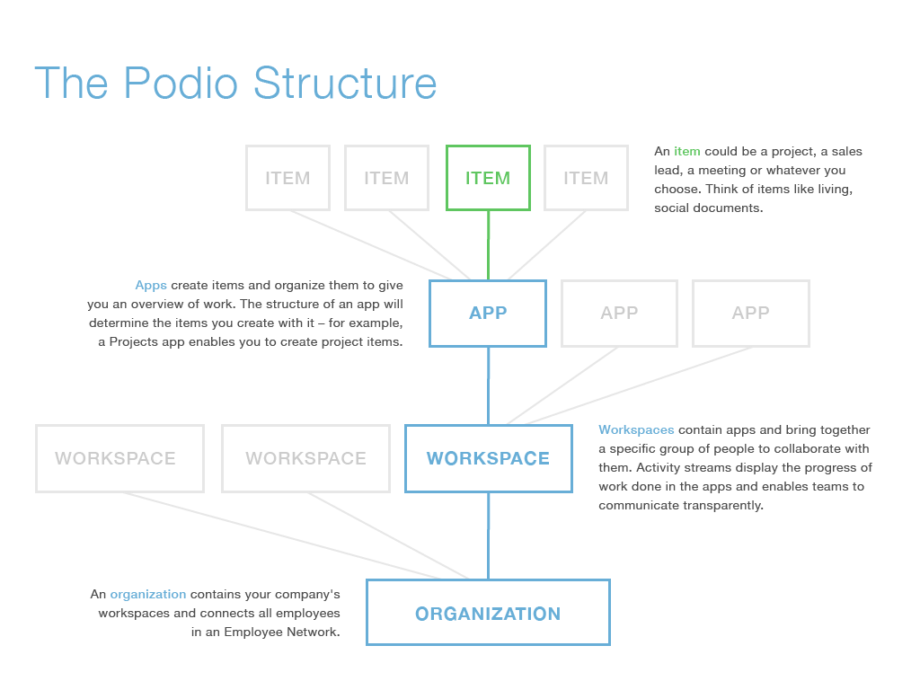
\includegraphics[width=\linewidth]{Podio_Structure.png}
    \caption{Algemene structuur van Podio \autocite{TallyfyPodio}. Geraadpleegd op 24 maart 2023, van https://tallyfy.com/what-is-podio.}
    \label{fig:podio_structure}
\end{figure}

In figuur \ref{fig:podio_structure} is te zien hoe Podio een organisatie opdeelt in drie groepen: Workspaces, Apps en Items. \\

Het doel van een workspace is om een groep mensen samen te brengen en van relevante apps te voorzien. Elke workspace bevat een activiteiten stroom, op die manier kan ieder groepslid zien wie wat gedaan heeft en wanneer dit gebeurd is \autocite{TallyfyPodio}. Workspaces worden vaak gebruikt om projecten of bedrijven te onderhouden. Er zijn drie types workspaces. Ten eerste is er de open workspace, deze is zichtbaar voor iedereen binnen een organisatie. Ten tweede is er de private workspace, dit type is initieel alleen zichtbaar voor de administrator van de organisatie, andere werknemers kunnen slechts toegang krijgen via een uitnodiging. Ten slotte is er nog de employee workspace, dit speciaal type workspace brengt elk lid van een organisatie samen via hun email domein. Zo heeft bijvoorbeeld iedereen met een @hogent.be email toegang tot de HOGENT workspace \autocite{PodioFeatures}. \\

Apps creëren meer overzicht binnenin een workspace en helpen het team hun werk op te volgen \autocite{PodioFeatures}. Elke app wordt opgebouwd uit een samenvoeging van bouwblokken of velden, deze staan gelijst in tabel \ref{tab:podio_velden}. Het belangrijkste veld in deze tabel is het 'Relationship' veld, want hiermee kunnen relaties gelegd worden tussen de verschillende apps. Bovendien heeft Podio ook een app store die bestaat uit pasklare apps, zo kunnen managers een volledig functionele applicatie opzetten in slechts enkele minuten tijd \autocite{TallyfyPodio}. \\

\begin{table}[ht]
    \centering
    \caption{\label{tab:podio_velden} Lijst met veld types voor Podio apps \autocite{PodioFeatures}.}
    \begin{tabular}{ | p{3cm} | p{11cm} | }
        \hline
        \textbf{Type} & \textbf{Beschrijving} \\
        \hline\hline
        Text & Wordt voor alles gebruikt. \\
        Category & Kan een bepaalde status bevatten en dus gebruikt worden voor filteren of sorteren. \\
        Date & Datum voor projecten of meetings instellen. \\
        Relationship & Wordt gebruikt om verschillende apps aan elkaar te koppelen via gedeelde data. \\
        Contact & Contactpersoon toevoegen aan een item. \\
        Number & Opnemen, rapporteren en berekenen van numerieke waarden. \\
        Link & Delen van links met bijhorende content previews. \\
        Image & Toevoegen van afbeeldingen zoals screenshots of designs. \\
        Money & Opnemen van geldwaarden om budget op te volgen en monetaire berekeningen te maken. \\
        Progress & Simpele progressie visualisatie. \\
        Calculation & Wordt gebruikt voor berekeningen en laat ook JavaScript toe. Dit type veld is een van de belangrijkste en word zeer vaak gebruikt, omdat er hele diverse zaken mee mogelijk zijn. \\
        Map & Locaties opnemen en weergeven via Google Maps. \\
        Duration & Opnemen van een tijdsspanne. \\
        \hline
\end{tabular}
\end{table}
    
% TODO Items - OK
Items worden aangemaakt door apps en kunnen in allerlei vormen voorkomen. Zo zal een project management app bijvoorbeeld projecten als items hebben. In een item wordt de inhoud over één onderwerp opgeslagen, het kan dus in essentie voorgesteld worden als een rij in een database. De manier waarop items gestructureerd zijn, kunnen een grote bijdrage hebben tot je ervaringen met Podio \autocite{TallyfyPodio}. \\

% TODO Quivvy - OK
Quivvy Solutions BV onderzoekt de business processen van hun klanten en welke tools zij daarvoor gebruiken. Hierna gaan ze deze processen gaan configureren in Podio. Daarbovenop onderzoeken ze ook welke tools van de klant gelinkt, of zelfs vervangen kunnen worden door Podio. Verder gaan ze afzonderlijke processen omzetten naar workflows en die, indien mogelijk, ook automatiseren \autocite{QuivvySoftware}. Kortom analyseert Quivvy Solutions de processen en gegevens van hun klanten en zetten deze vervolgens om naar een Podio-omgeving waarmee de klant in staat is om zijn volledige bedrijfsinfrastructuur te beheren. \\

\subsection{Podio API}
\label{subsec:podio_API}

% TODO Podio API - OK
% TODO Bronnen Toevoegen - OK

Podio frontend werd volledig gebouwd op zijn Application Programming Interface of kortom API. Hierdoor is het platform gemakkelijk uit te breiden en biedt het tal van mogelijkheden, zo heeft men bijvoorbeeld de mogelijkheid om webhooks te registreren in Podio apps \autocite{PodioAPI2023}. Webhooks zorgen ervoor dat een bepaalde URL kan aangeroepen worden wanneer een item wordt aangemaakt, aangepast of verwijderd wordt in Podio. Hierdoor kunnen gebruikers event-driven apps bouwen, zoals bijvoorbeeld een notificatie systeem via SMS \autocite{PodioAPIWebhooks}. \\

Momenteel wordt de API voorzien in PHP, .NET, Ruby, Java, Python, Android en Objective-C. Om de API te kunnen gebruiken heeft een gebruiker een API key nodig en moet ze OAuth geauthenticeerd zijn. De Podio API past het RESTful principe toe en gebruikt JSON als zijn uitwisselingsformaat. Vervolgens maakt het gebruik van volgende HTTP methoden om data te manipuleren: GET (ophalen), POST (aanmaken), PUT (bewerken) en DELETE (verwijderen). Bovendien is de API slash-aware, dit betekent dat een URL die eindigt met een schuine streep niet hetzelfde is als een URL zonder het teken. De streep wordt enkel toegevoegd als de bron een lijst van data is \autocite{PodioAPIConcepts}. \\


\subsection{Extensies}
\label{subsec:podio_extensies}

% TODO Bronnen Toevoegen - OK

Het feit dat Podio op zijn API gebouwd is, laat third-party developers toe om hun eigen uitbreidingen of extensies te bouwen op Podio. Deze extensies kunnen heel diverse doeleinden hebben, ze voegen niet alleen extra functionaliteiten toe, maar kunnen ook bestaande processen verbeteren \autocite{PodioExtensions}. Zo is er bijvoorbeeld GlobiMail, dat automatisch e-mails vanuit de inbox neemt en toevoegt als commentaar aan Podio items. Een tweede voorbeeld is SmartGantt, dat toelaat om data te visualiseren in Gantt grafieken. Elke gebruiker kan suggesties doen of zelf extensie bouwen en die presenteren aan het Podio team. \\

% https://podio.com/extensions/5
% https://podio.com/extensions/3


\subsection{Workflow Automations (Globiflow)}
\label{subsec:workflow_automations}

% TODO Workflow Automation - OK
% TODO Bronnen aanvullen - OK
Citrix Podio Workflow Automation, vroeger Globiflow genoemd, laat toe om belangrijke taken en processen te automatiseren, om op die manier tijd en geld te besparen. Via triggers kunnen een groot aanbod aan functies uitgevoerd worden op een vastgezet tijdstip of na een bepaalde actie \autocite{PodioWorkflowAutomation}. Elke workflow bestaat uit een trigger, filters en minstens één actie. Triggers kunnen allerlei zaken zijn zoals een bepaald tijdstip, een Podio item die aangemaakt of upgedate wordt, een bepaalde filter, ... \autocite{PodioWorkflowFeatures}. \\

De voornaamste acties die gebruikt worden in workflows zijn;
\begin{itemize}
    \item \textit{E-mails of sms-berichten verzenden}: Via deze actie kan men emails of SMS berichten verzenden naar externen. Deze kunnen zelf vooraf opgesteld worden en informatie naar keuze uit Podio items bevatten. Een antwoord op het bericht kan ook gebruikt worden als trigger voor een andere workflow. \autocite{PodioWorkflowFeatures}
    \item \textit{pdf-bestanden genereren}: Informatie uit Podio items kan automatisch omgezet worden naar een PDF bestand en indien nodig toegevoegd worden aan emails. Dit kan bijvoorbeeld handig zijn voor het automatiseren van opstellen en verzenden van facturen. \autocite{PodioWorkflowFeatures}
    \item \textit{Embedden in een website}: Door een simpele script tag toe te voegen aan de bron van de website kan data uit Podio items weergegeven worden op de site zelf. Op die manier kan Podio dus gebruikt worden als een eenvoudig Content Management System (CMS). \autocite{PodioWorkflowFeatures}
    \item \textit{Data visualiseren in grafieken}: Een rapport kan via workflows eenvoudig omgezet worden in een grafiek zoals een lijndiagram, taartdiagram, ... Deze grafieken kunnen vervolgens als afbeeldingen weergegeven worden op dashboards in Podio. \autocite{PodioWorkflowFeatures}
    \item \textit{Data feeds}: Soms is het ook belangrijk om data uit Podio te halen en deze te gebruiken in een externe applicatie. Data kan omgezet worden in JSON of XLM en zo doorgegeven worden. \autocite{PodioWorkflowFeatures}
\end{itemize}

\section{Airtable}
\label{sec:airtable}

% TODO Airtable (DRAFT) - OK
% TODO Airtable (FINAL) - 

\subsection{Ontstaan van Airtable}
\label{subsec:ontstaan_airtable}

% https://builtonair.com/a-brief-history-of-airtable/
% https://nira.com/airtable-history/
% TODO Bronnen Toevoegen - OK

Het idee achter Airtable werd bedacht door Howie Liu in 2012. Hij zag in dat spreadsheets enkel als simpele opslag werden gebruikt, terwijl ze zoveel meer te bieden hadden. Samen met mede-oprichter Andrew Ofstand bouwden ze het idee uit tot een eenvoudig prototype, dat ze dan presenteerden aan Amerikaanse acteur Aston Kutcher. Hij besloot direct te investeren, waardoor Airtable officieel gelanceerd werd en begon met development. Twee jaar later, in 2014, starte de open-beta van de app, die toen zeer goed ontvangen werd door de eerste gebruikers \autocite{Black2019}.
Airtable behield dit momentum en bracht in de komende jaren tal van features uit zoals views, integraties en eigen Airtable API \autocite{Shah}. \\

\subsection{Wat is Airtable?}
\label{subsec:wat_is_airtable}

% TODO Bronnen Toevoegen - OK

Airtable is een low-code/no-code platform waarmee gebruikers op maat gemaakte applicaties kunnen bouwen zonder enige programmeervaardigheden. Het laat toe om eenvoudig een interne database te creëren die belangrijke informatie voor het werk bevat. Bovenop deze database kan dan een krachtige applicatie gebouwd worden die ook workflows en projecten automatiseert. Met Airtable kunnen gebruikers alle informatie met betrekking tot hun doelen en doelstellingen bijhouden en koppelen aan andere tools voor het automatiseren van taken, zoals het verzenden van een email. Automatisaties kunnen getriggerd worden door specifieke acties of tijdstippen. Hierdoor kan men tijd besparen op repetitieve taken en zich focussen op zaken die belangrijker zijn. Daarnaast maakt het platform ook eenvoudige weergave van gegevens mogelijk, via Gantt-grafieken of andere soorten visualisaties. Airtable brengt informatie uit verschillende bronnen samen en stelt gebruikers in staat hun gegevens te sorteren, te filteren en te herschikken om zo aangepaste views (zie \ref{fig:exampleairtable}) voor hun teamleden en partners te creëren. Op die manier heeft iedere stakeholder de informatie die voor hen het meest noodzakelijk is. Het platform biedt gebruikers volledige controle over de applicaties die ze bouwen, ongeacht hun programmeerkennis, dankzij de flexibele en krachtige database die is afgestemd op complexe en specifieke workflows \autocite{AirtableWhat}. \\

% TODO Fig Voorbeeld invoegen https://www.airtable.com/guides/start/what-is-airtable - OK
\begin{figure}
    \centering
    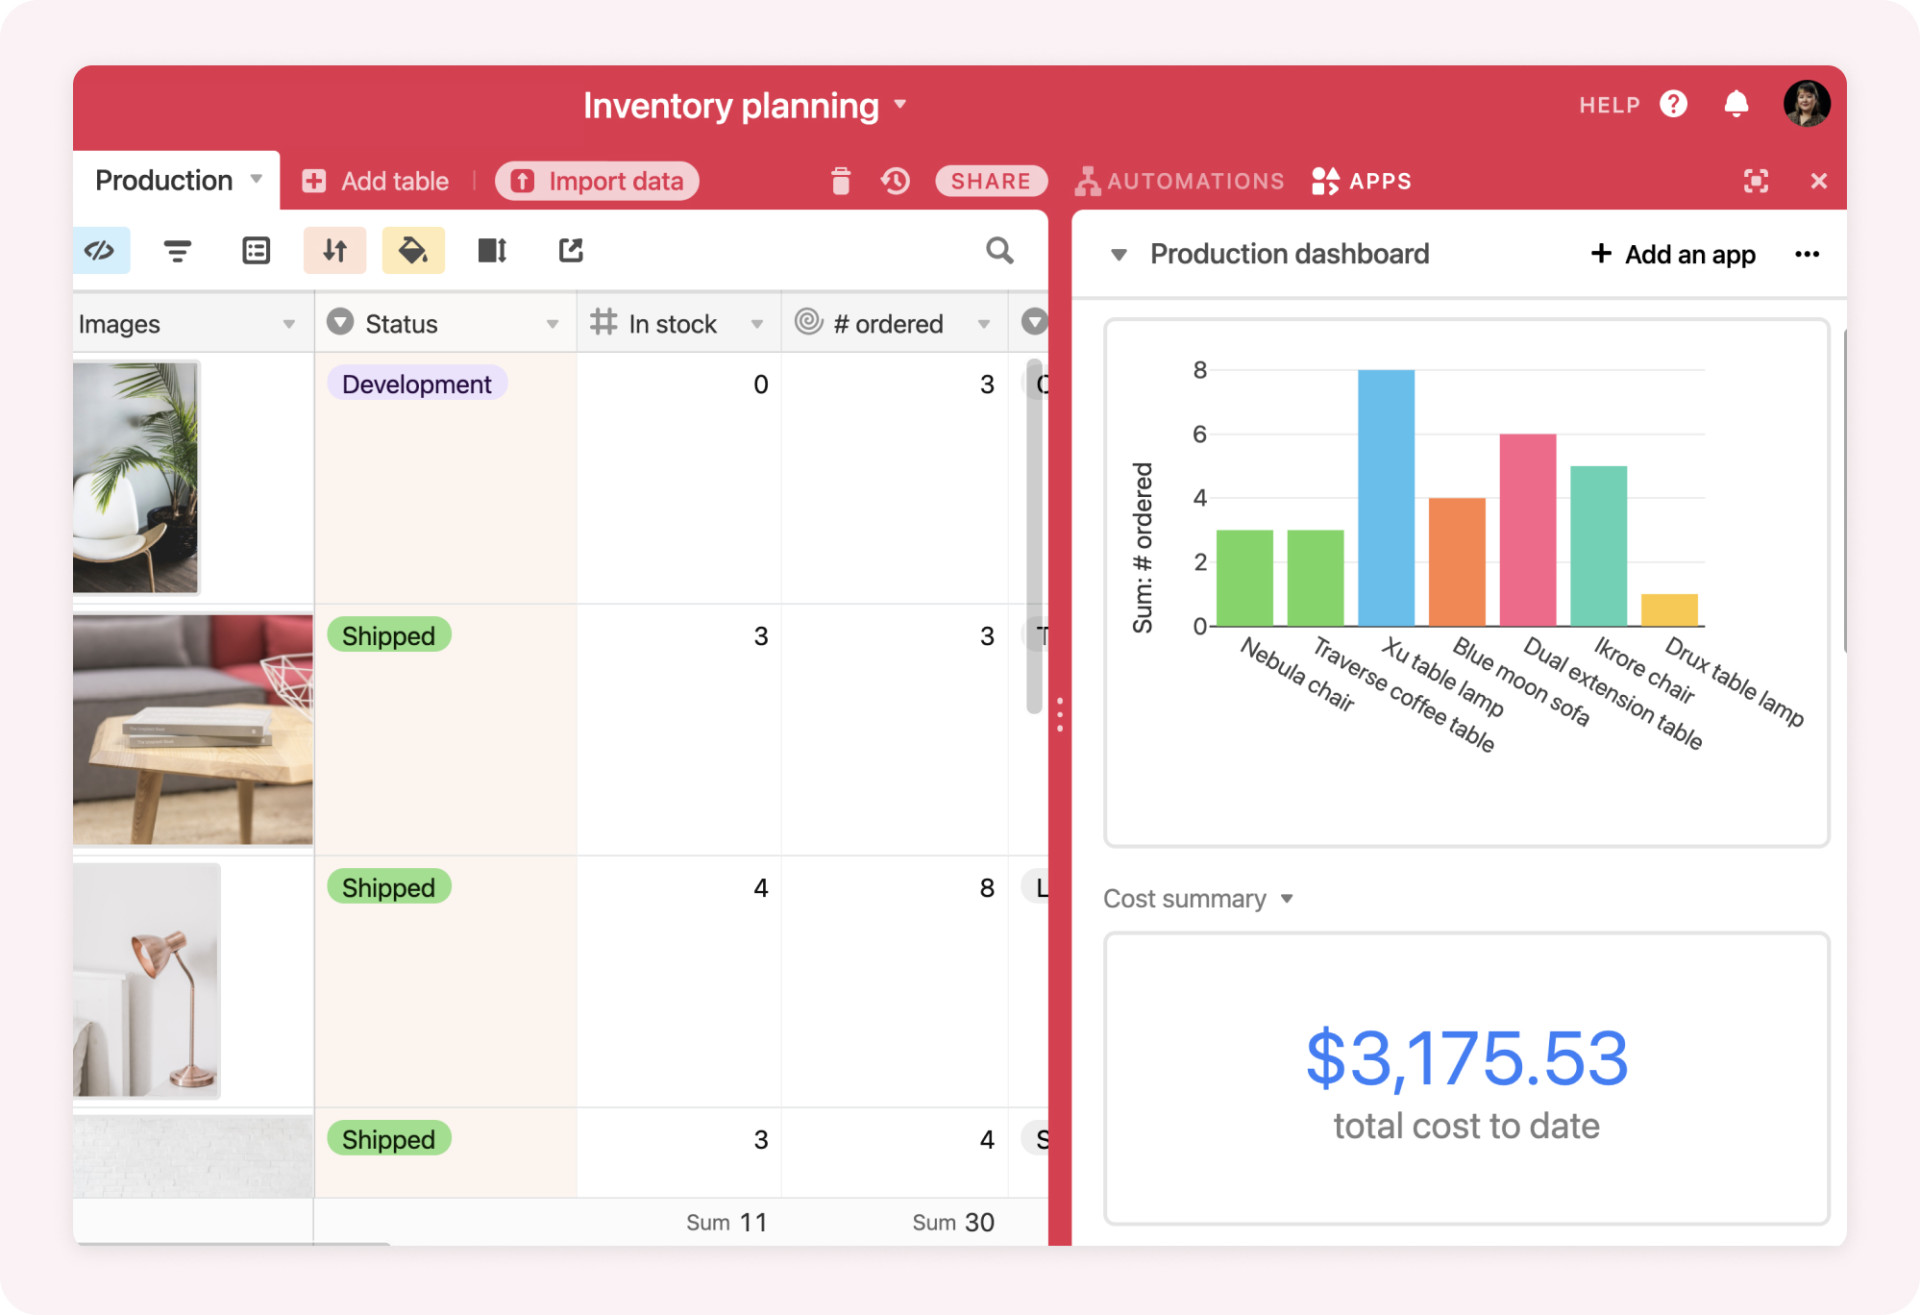
\includegraphics[width=\linewidth]{Airtable_WatIs_Voorbeeld.jpg}
    \caption{Voorbeeld van Airtable view \autocite{AirtableWhat}.}
    \label{fig:exampleairtable}
\end{figure}

Het kernidee van Airtable draait rond het gebruik van een `Single source of truth` of enkele bron van waarheid, die in real-time up-to-date gehouden wordt. Veel processen ondervinden vertragingen 
wanneer men dezelfde informatie meermaals moet gaan bijwerken op verschillende plaatsen. Dit leidt niet alleen tot frustratie, maar soms ook tot fouten, die kunnen resulteren in erge gevolgen. Met Airtable wordt alle data gecentraliseerd en gesynchroniseerd, waardoor het bijwerken van data slechts één keer moet gebeuren. Zo weet elk teamlid dat ze altijd met de meest actuele informatie werken en kunnen eventuele fouten vermeden worden \autocite{AirtableWhat}. \\

\subsection{Airtable Web API}
\label{subsec:airtable_web_API}

% TODO Bronnen Toevoegen - OK

Om data te integreren met externe applicaties of systemen wordt gebruik gemaakt van de Airtable Web API. Alhoewel de officiële client gebouwd is in JavaScript, zijn er ook community-built versies beschikbaar in Ruby, .NET, Python 3 en Python 2/3. De API houdt zich aan REST semantiek, gebruikt JSON om objecten te encoderen, en steunt op standaard HTTP codes om resultaten van operaties aan te tonen \autocite{AirtableAPI}. Met deze API kan men data lezen, creëren, updaten en verwijderen. \\

Airtable WEB API maakt gebruik van token-based authenticatie. Dit betekent dat alle requests een persoonlijke of OAuth token in hun header moeten hebben, zoals in figuur \ref{fig:airtable_authtoken} weergegeven \autocite{AirtableAPIAuthentication}. \\

% TODO Fig Auth token invoegen - OK
% TODO Fig Voorbeeld invoegen https://www.airtable.com/guides/start/what-is-airtable - OK
\begin{figure}
    \centering
    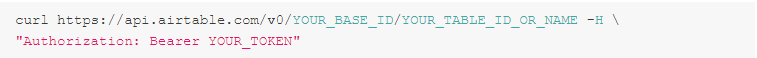
\includegraphics[width=\linewidth]{Airtable_WebAPI_AuthToken.png}
    \caption{Voorbeeld van Airtable API call \autocite{AirtableAPIAuthentication}. Geraadpleegd op 29 maart 2023, van https://airtable.com/developers/web/api/scopes.}
    \label{fig:airtable_authtoken}
\end{figure}

Scopes bepalen welke acties de gebruiker kan uitvoeren en zitten verwerkt in de access token. Er zijn drie verschillende soorten scopes in de Airtable Web API, namelijk `Basic scopes`, `Enterprise member scopes` en `Enterprise admin scope`. Hierbij omvat de `Basic scopes` het minste aantal acties en `Enterprise admin scopes` de meeste. Het is belangrijk om te vermelden dat, om data te bewerken, de gebruiker zowel de juiste scope als toegang tot de data moet hebben. \autocite{AirtableAPIScopes}. \\

\section{(Google) AppSheet}
\label{sec:Appsheet}

% TODO AppSheet (DRAFT) - OK
% TODO AppSheet (FINAL) - 


\subsection{Wat is AppSheet?}
\label{subsec:wat_is_appsheet}

AppSheet is een no-code development platform dat werd overgenomen door Google in 2020. Het laat toe om mobiele en desktop applicaties te bouwen zonder enige code te hoeven schrijven. Het maakt gebruik van spreadsheets en databases zoals SQL of AWS om automatisch data te visualiseren. Deze weergaven zijn bovendien volledig bewerkbaar door gebruiker zelf \autocite{AppSheet2020}. AppSheet is vooral nuttig voor zakelijke use cases zoals CRM, projectbeheer en gepersonaliseerde rapporten. Het biedt geavanceerde machine learning en AI-functies, waaronder waardevoorspelling, OCR, sentimentanalyse en anomaliedetectie. AppSheet is gratis voor prototyping en persoonlijk gebruik, maar voor commerciële toepassingen is een maandelijks bedrag vereist. Bovendien zijn een actieve internetverbinding en een client app nodig om toegang te krijgen tot AppSheet applicaties en hun functies, aangezien ze in de cloud worden ingezet \autocite{Petrovic2020}. \\

\subsection{AppSheet Templates}
\label{subsec:appsheet_templates}

% TODO Bronnen Toevoegen - OK

AppSheet voorziet een groot aanbod aan templates voor verschillende use cases. In tabel \ref{tab:Tabel 2} werden enkele voorbeelden gelijst, die aantonen dat het platform voor zeer diverse doeleinden gebruikt kan worden. 

\begin{table}[ht]
    \centering
    \caption{\label{tab:Tabel 2} Lijst met beschikbare AppSheet templates \autocite{AppSheetTemplates}.}
    \begin{tabular}{ | p{5cm} | p{9cm} | }
        \hline
        \textbf{Template} & \textbf{Beschrijving} \\
        \hline\hline
        Simple Survey & basisstructuur voor formulieren of vragenlijsten aan te maken \\
        Simple Inventory & Bijhouden en monitoren van een opslag \\
        Kanban Board & Projecten en taken opvolgen in een kanban dashboard \\
        Workstation Booking & Reserveren en toewijzen van deelbare ruimtes binnen een organisatie \\
        Order Deliveries & Opvolgen en klanten op de hoogte houden van leveringen \\
        Task Manager & Opvolgen van (herhalende) taken \\
        Facility Assets & Opvolgen van activa binnen een bedrijf \\
        Occupancy Tracker & Opvolgen van de beschikbaarheid van bepaalde kamers of ruimtes \\
        Client Expenses & Opvolgen en sorteren van uitgaven gemaakt door klanten \\
        To Do List & Simpele to do lijst die opgedeeld kan worden in categorieën \\
        Shift Scheduling & Roosteren en onderhouden van shifts voor bedrijfsmedewerkers \\
        Incident Report & Melden en rapporteren van incidenten. \\
        Route Optimization & Routes plannen voor chauffeurs a.d.h.v. Google Maps API \\
        Events Calendar &  Evenementen organiseren op een gedeelde kalender \\
        Contact Manager & Onderhouden en loggen van persoonlijke of business contacten en interacties \\
        \hline
    \end{tabular}
    \vspace{0.3cm}
    {\raggedright \textit{Opm. Deze lijst beperkt zich tot slechts 15 templates} \par}
\end{table}

\subsection{Opzetten van een eenvoudige applicatie in AppSheet}
\label{subsec:opzetten_applicatie_appsheet}

% TODO Bronnen Toevoegen - OK

Het bouwen van een envoudige applicatie in AppSheet gaat als volgt. Eerst en vooral moet men data voorzien. Het platform ondersteunt verscheidene soorten data bronnen zoals Excel, Cloud SQL, etc. De omschrijving van de data moet in de eerste rij worden geplaatst, op die manier kan AppSheet de data uit elkaar houden. Daarna wordt de data aan de applicatie verbonden, Appsheet host namelijk zelf geen data, maar interageert er enkel mee. Vervolgens moet gedefiniëeerd worden hoe de data gebruikt zal worden, er kan bijvoorbeeld voor gekozen worden om bepaalde data niet weer te geven of om een formule erop toe te passen vooraleer het in de applicatie getoond wordt. Na deze stap word User Interface (UI) opgemaakt, deze bestaat uit views. AppSheet voorziet een hele reeks aan pasklare views die gebruikt en aangepast kunnen worden.  Daarna kan men bots toevoegen om automatisaties te runnen zoals bijvoorbeeld het verzenden van een email. Een bot bestaat uit drie componenten: een event, een taak en een proces. Een event kan gelijkgesteld worden aan een trigger in Podio, het bepaald namelijk wanneer een bot zijn taak moet gaan uitvoeren. Een taak is de actie die moet uitgevoerd worden nadat een event is getriggered. Via een process kunnen verschillende taken opgedeeld worden in stap met eventuele conditionele logica. Ten slotte hoeft men de gemaakte applicatie alleen nog maar te deployen. AppSheet zal nog enkele checks uitvoeren om na te gaan of de app proper werkt en vervolgens live zetten. De applicatie kan dan gedownload worden of geopend worden in een web browser \autocite{AppSheetHowToCreate}. \\
